\section{Results}\label{sec:results}
\subsection{The primary intervention changes judged style but fails preservation}
\Tabref{tab:primary} reports the two-seed primary comparison. Mean $-2$ reduces judge AI-likeness by 20.039 points (CI $[-22.852,-17.266]$; Holm $p=0.00020$; $d_z=-1.728$). The encoder changes by $+0.061$ (CI $[-0.072,+0.193]$; Holm $p=0.381$), providing no corroboration of the primary reduction.

Coherence falls by 0.591 points, with its entire CI below the $-0.25$ preservation margin. This is clear coherence damage. Coverage changes by $-0.0279$, but its lower bound $-0.0573$ also fails the $-0.05$ gate; this interval leaves preservation inconclusive rather than establishing a loss beyond the margin. Unsupported claims change by $+0.0141$, with an interval spanning zero. Thus, neither primary quality gate passes.
\begin{table}[t]
\centering\small
\caption{Primary instruction contrast: mean $-2$ versus zero, averaging two seeds within each of 64 records. CIs are paired prompt-bootstrap 95\% intervals. Only the two style $p$-values receive Holm correction. Lower style scores alone do not establish improvement; neither preservation gate passes.}\label{tab:primary}
\resizebox{\textwidth}{!}{\begin{tabular}{@{}lrrlrr@{}}
\toprule
Outcome & Zero & Mean $-2$ & Change [95\% CI] & Holm $p$ & $d_z$\\
\midrule
Encoder probability & 0.476 & 0.537 & $+0.061\;[-0.072,+0.193]$ & 0.381 & $+0.112$\\
Judge AI-likeness & 69.219 & 49.180 & $-20.039\;[-22.852,-17.266]$ & 0.00020 & $-1.728$\\
Coherence & 4.703 & 4.112 & $-0.591\;[-0.754,-0.427]$ & --- & $-0.888$\\
Fact coverage & 0.919 & 0.891 & $-0.0279\;[-0.0573,+0.0016]$ & --- & $-0.229$\\
Unsupported claims & 0.179 & 0.193 & $+0.0141\;[-0.0137,+0.0422]$ & --- & $+0.121$\\
\bottomrule
\end{tabular}}
\end{table}


\para{Signed doses expose measurement disagreement.}
Positive mean $+2$ raises judge AI-likeness by 16.93 points (CI $[15.10,18.72]$) while lowering encoder probability by 0.459 (CI $[-0.545,-0.373]$). Coherence falls by 0.414 and coverage by 0.131. \Figref{fig:dose} shows the seed-42 curve; intermediate instruction doses show that score and quality changes depend on magnitude. The two style measures are not interchangeable operationalizations of AI-like writing.
\begin{figure}[t]\centering
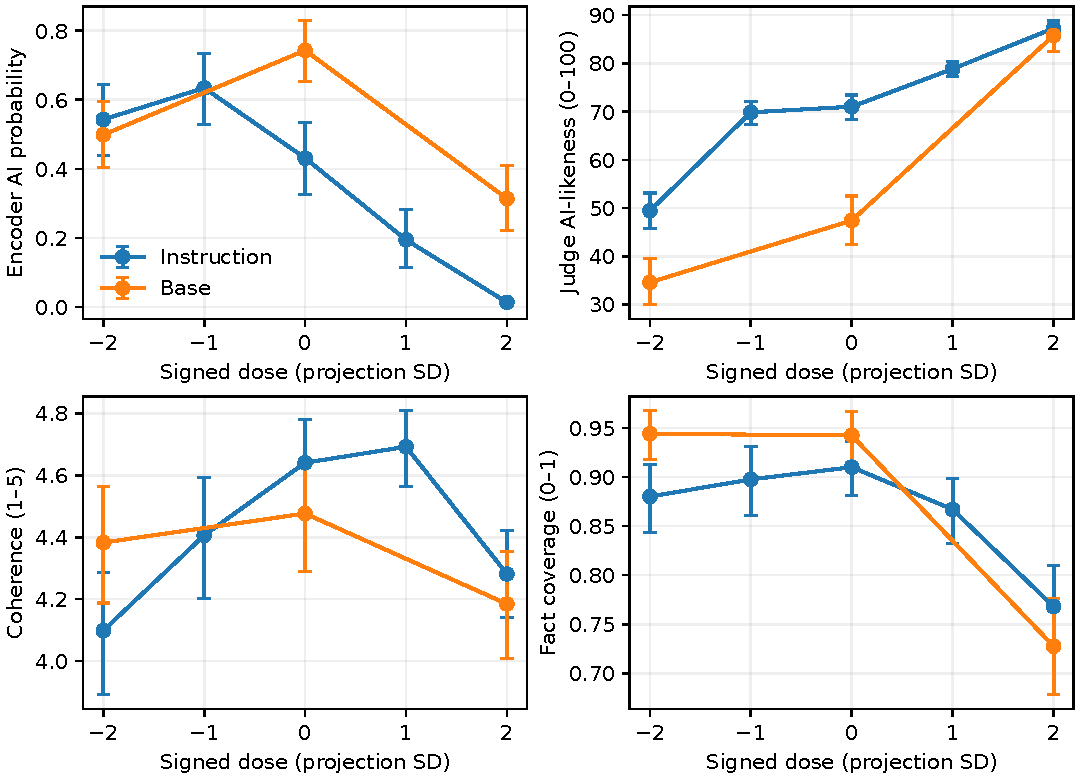
\includegraphics[width=0.95\linewidth]{figures/dose_response.pdf}
\caption{Signed-dose response at seed 42: means and prompt-bootstrap 95\% intervals over 64 tasks per point. Base observations exist only at $-2$, 0, and $+2$; connecting lines do not imply tested intermediate doses. The primary analysis in \tabref{tab:primary} instead averages two seeds. Judge style changes accompany quality costs and diverge from encoder scores.}\label{fig:dose}
\end{figure}

\subsection{Random, nuisance, ablation, and prompt controls}
\Tabref{tab:controls} reports all instruction condition families. At seed 42, mean $-2$ lowers the judge score 23.08 points more than the average of five random directions (CI $[-26.44,-19.55]$), with an additional coherence loss of 0.493. Its encoder contrast against the random average is $-0.012$ (CI $[-0.129,+0.107]$). Generic equal-norm perturbation therefore does not explain the large judged effect, but the encoder does not establish the corresponding specific change.
\begin{table}[t]
\centering\small
\caption{Instruction-model changes relative to the same-seed zero baseline. Mean $\pm2$ averages two seeds; all other conditions use seed 42. The random row is a range across five conditions. No intervention is an overall winner across style and preservation. Full individual intervals appear in \secref{sec:extended}.}\label{tab:controls}
\begin{tabular}{@{}lrrrr@{}}
\toprule
& \multicolumn{2}{c}{Style score change} & \multicolumn{2}{c}{Quality change}\\
\cmidrule(lr){2-3}\cmidrule(lr){4-5}
Condition & Judge & Encoder & Coherence & Coverage\\
\midrule
Mean $-1$ & $-1.17$ & $+0.203$ & $-0.234$ & $-0.013$\\
Mean $-2$ & $-20.04$ & $+0.061$ & $-0.591$ & $-0.028$\\
Mean $+1$ & $+7.84$ & $-0.237$ & $+0.052$ & $-0.043$\\
Mean $+2$ & $+16.93$ & $-0.459$ & $-0.414$ & $-0.131$\\
Logistic $-2$ & $-15.39$ & $+0.214$ & $-0.570$ & $-0.039$\\
Projection ablation & $-15.78$ & $+0.223$ & $-0.233$ & $-0.002$\\
Random (five) & $[-3.05,+3.91]$ & $[+.043,+.219]$ & $[-.164,+.148]$ & $[-.025,+.016]$\\
Formality $-2$ & $+1.88$ & $-0.159$ & $+0.063$ & $-0.071$\\
Assistant proxy $-2$ & $+4.77$ & $-0.259$ & $+0.125$ & $-0.051$\\
Residualized $-2$ & $-8.67$ & $+0.196$ & $-0.555$ & $-0.045$\\
Residualized $+2$ & $+13.00$ & $-0.327$ & $-0.406$ & $-0.111$\\
Human-style prompt & $-6.02$ & $-0.126$ & $-0.094$ & $-0.024$\\
\bottomrule
\end{tabular}
\end{table}


Logistic steering and projection ablation also reduce judged AI-likeness, by 15.39 and 15.78 points, while increasing encoder scores. Ablation nearly preserves mean coverage ($-0.002$), and its coverage interval passes that gate, but its coherence interval does not pass. The human-style prompt produces a smaller judge reduction ($-6.02$) and an encoder reduction ($-0.126$); neither preservation gate is established at this sample size.

\para{Does nuisance removal isolate AI style?}
Instruction-direction cosines are $-0.038$ with formality, $+0.039$ with verbosity, $-0.236$ with assistant persona, $-0.231$ with length, and $+0.072$ with domain. Joint removal retains 86.3\% of vector norm and GPT-4o test AUROC 0.966. Residualized $-2$ still reduces judge AI-likeness by 8.67 points, but lowers coherence by 0.555 and increases encoder score by 0.196. This excludes simple collinearity with the measured proxies, not semantic dependence on the underlying constructs. \Figref{fig:controls} provides the full control contrasts.

\subsection{Readout transfers unevenly and is not amplified by instruction tuning}
\Tabref{tab:transfer} separates the backbone used to read text from the generator that wrote it. Held-out GPT-4o AUROC is 0.9707 for the base backbone and 0.9704 for the instruction backbone. Their paired instruction-minus-base difference is $-0.0003$ (CI $[-0.0051,+0.0053]$). We find no amplification in this metric; this is not an equivalence test for every aspect of representation strength.
\begin{table}[t]
\centering\small
\caption{Validation-selected mean-direction AUROC on 128 human/machine pairs per row. Backbone is the model extracting representations; generator produced the comparison text. Bold marks the numerically higher backbone AUROC per row, not a significant difference. Human references are shared across generators within source sets.}\label{tab:transfer}
\begin{tabular}{@{}llrr@{}}
\toprule
Corpus / domains & Generator & Base backbone & Instruction backbone\\
\midrule
\textsc{HAP-E}, academic/blog/news & GPT-4o & \textbf{0.971} & 0.970\\
& Llama-3-8B base & 0.479 & \textbf{0.486}\\
& Llama-3-8B instruction & 0.912 & \textbf{0.913}\\
\textsc{HAP-E}, held-out domains & GPT-4o & \textbf{0.975} & 0.973\\
& Llama-3-8B base & 0.549 & \textbf{0.564}\\
& Llama-3-8B instruction & \textbf{0.913} & 0.911\\
\textsc{HC3}, question answers & ChatGPT & \textbf{0.923} & 0.909\\
\bottomrule
\end{tabular}
\end{table}


For the instruction backbone, in-domain GPT-4o AUROC has CI $[0.950,0.987]$. Transfer to Llama-3 instruction outputs remains strong (0.913), but Llama-3 base outputs are near chance (0.486; CI $[0.423,0.550]$). Held-out domains and \hcthree retain substantial readout performance. These are readout-transfer results, not demonstrations of causal transfer to those tasks.

Base-model negative steering lowers both judge AI-likeness by 12.81 (CI $[-18.28,-7.03]$) and encoder score by 0.244 (CI $[-0.365,-0.124]$). Its coherence change is $-0.094$ (CI $[-0.320,+0.133]$), which still fails the noninferiority gate. We did not run the extended controls on the base model, and prompt formats differ across checkpoints.

\para{Partial length and fluency checks.}
Restricting within-pair token-length differences to at most ten retains instruction AUROC 0.973 on 64 in-domain pairs and 0.976 on 77 held-out-domain pairs. Training projections correlate $-0.075$ with token length and $-0.313$ with model negative log likelihood (NLL). Negative NLL achieves 0.684 AUROC for in-domain GPT-4o, compared with 0.970 for the mean direction, but reaches 0.903 for Llama base where the mean direction is near chance. These checks do not establish independence from length or fluency.

\subsection{Measurement validity and robustness qualify the causal finding}
On 64 held-out \hape human/GPT-4o pairs, encoder AUROC is 0.656 (CI $[0.585,0.729]$), with human/AI mean scores 0.033/0.155. Judge AUROC is 0.965 (CI $[0.930,0.992]$), with means 17.42/58.05. The encoder transfers weakly under this domain/generator shift. Its disagreement limits corroboration rather than decisively refuting every style effect. Across generated outputs, encoder/judge Spearman correlation is $-0.375$.

On 64 re-rated outputs, judge AI-likeness rank agreement is 0.661 and mean absolute difference is 10.78 points; coherence agreement is 0.850 with mean absolute difference 0.211. No human-rating validation was performed. Calibration discriminating known provenance does not validate every treatment-induced style distinction.

The negative judge effect appears at both seeds ($-21.56$ and $-18.52$), with coherence loss at both. Resampling eight topic/template clusters yields judge CI $[-22.70,-17.30]$ and coherence CI $[-0.793,-0.405]$; eight clusters provide limited population coverage. Exploratory length adjustment leaves a judge coefficient near $-20.45$, which is not an identified direct effect.

Matched-quality filtering retains only 11/64 instruction pairs at seed 42. Their judge change is $-15.45$ (CI $[-28.64,-1.82]$), while the encoder change is $+0.301$ (CI $[-0.032,+0.613]$). Only 22 base pairs pass the same filter, with both scores lower. These selected subsets cannot establish preservation for all prompts; small-sample bootstrap and discrete sign-flip inference can also differ.
